\newcommand{\NWtarget}[2]{\hypertarget{#1}{#2}}
\newcommand{\NWlink}[2]{\hyperlink{#1}{#2}}
\newcommand{\NWtxtMacroDefBy}{Fragment defined by}
\newcommand{\NWtxtMacroRefIn}{Fragment referenced in}
\newcommand{\NWtxtMacroNoRef}{Fragment never referenced}
\newcommand{\NWtxtDefBy}{Defined by}
\newcommand{\NWtxtRefIn}{Referenced in}
\newcommand{\NWtxtNoRef}{Not referenced}
\newcommand{\NWtxtFileDefBy}{File defined by}
\newcommand{\NWtxtIdentsUsed}{Uses:}
\newcommand{\NWtxtIdentsNotUsed}{Never used}
\newcommand{\NWtxtIdentsDefed}{Defines:}
\newcommand{\NWsep}{${\diamond}$}
\newcommand{\NWnotglobal}{(not defined globally)}
\newcommand{\NWuseHyperlinks}{}
\documentclass[12pt, english, oneside]{report}
\usepackage[a4paper, left=1cm, right=1cm, top=3cm, marginparwidth=2cm]{geometry}
\usepackage{marginnote}

\setcounter{secnumdepth}{3} % default value for 'report' class is "2"


\usepackage[utf8]{inputenc}
\usepackage[T1]{fontenc}
\usepackage{tikzsymbols}
\usepackage[backend=bibtex, style=numeric, sorting=none]{biblatex} 
\usepackage{csquotes}
\setlength\bibitemsep{\baselineskip}
\addbibresource{References.bib}

\usepackage{float} % to take away the error unknown float option `H'
% https://stackoverflow.com/a/27243065/505306
% Making caption font smaller on figures and tables.
\usepackage{caption}
\captionsetup{font=footnotesize}

%-------------------------------------------------------------------------------
%\usepackage[left,pagewise]{lineno}
%\usepackage[right]{lineno}
%\linenumbers
%--------------------------------------------------------------------------------
\usepackage[framemethod=TikZ]{mdframed}
\usepackage{wrapfig}
\usepackage{amsthm}
\usepackage{amsfonts}
% ------------------------------------------------------------------------------
\usepackage[toc,page]{appendix}
\usepackage[stretch=10]{microtype} % https://tex.stackexchange.com/a/586  The great microtype package
%-------------------------------------------------------------------------------
%https://tex.stackexchange.com/a/278199/17858
% For aligning itemize environments to left
\usepackage{enumitem}
\mdfsetup{%
   middlelinecolor=red,
   middlelinewidth=0pt,
   roundcorner=10pt}

\mdfdefinestyle{MyFrame}{%
    linecolor=black,
    outerlinewidth=0.1pt,
    roundcorner=0pt,
    innertopmargin=14pt,
    innerbottommargin=4pt,
    innerrightmargin=4pt,
    innerleftmargin=4pt,
        leftmargin = 4pt,
        rightmargin = 4pt,
    %backgroundcolor=gray!50!white}
     }
%-------------------------------------------------------------------------------

\definecolor{theocol}{RGB}{255, 222, 228}
\newtheorem{theo}{Theorem}
\newenvironment{ftheo}
  {\begin{mdframed}[style=MyFrame,nobreak=true, backgroundcolor=theocol]\begin{theo}}
  {\end{theo}\end{mdframed}}


\definecolor{lemcol}{RGB}{226, 255, 220}
\newtheorem{lem}{Lemma}
\newenvironment{flem}
  {\begin{mdframed}[style=MyFrame,nobreak=true, backgroundcolor=lemcol]\begin{lem}}
  {\end{lem}\end{mdframed}}

\definecolor{corcol}{RGB}{227, 227, 227}
\newtheorem{cor}{Corollary}
\newenvironment{fcor}
  {\begin{mdframed}[style=MyFrame,nobreak=true, backgroundcolor=corcol]\begin{cor}}
  {\end{cor}\end{mdframed}}

\definecolor{propcol}{RGB}{227, 227, 227}
\newtheorem{prop}{Proposition}
\newenvironment{fprop}
  {\begin{mdframed}[style=MyFrame,nobreak=true, backgroundcolor=propcol]\begin{prop}}
  {\end{prop}\end{mdframed}}

\definecolor{conjcol}{RGB}{248, 218, 194}
\newtheorem{conj}{Conjecture}
\newenvironment{fconj}
  {\begin{mdframed}[style=MyFrame,nobreak=true, backgroundcolor=conjcol]\begin{conj}}
  {\end{conj}\end{mdframed}}


\definecolor{notecol}{RGB}{255, 152, 149  }
\newenvironment{note}
  {\begin{mdframed}[style=MyFrame,nobreak=true, backgroundcolor=notecol]}
  {\end{mdframed}}

\usepackage{enumitem}

%-------------------------------------------------------------------------------
% https://tex.stackexchange.com/q/2291/17858
% if you want to create a new list from scratch
\newlist{alphalist}{enumerate}{1}
% in that case, at least label must be specified using \setlist
\setlist[alphalist,1]{label=\textbf{\Alph*.}}

%--------------------------------------------------------------------------------
\usepackage[english]{babel}
%\setlength{\voffset}{-0.75in}
\setlength{\headsep}{5pt}

%-------------------------------------------------------------------------------
\usepackage{blindtext}
\usepackage{lipsum}
\usepackage{kantlipsum}
\usepackage{textcomp}

\usepackage{amssymb}
\usepackage{amsmath}
\usepackage{IEEEtrantools}
\usepackage{mathtools}

\usepackage{listings}


%-----------------------------------------------------------------------------------------------
\usepackage[inline]{asymptote}
\usepackage{asypictureB}
\usepackage{filecontents}
\usepackage{parskip} 
\usepackage{tocloft}
\usepackage{graphicx}                             % Include images into pdf document 
\usepackage{tikz}                                 % Useful for the circled command. Don't remove!
\usepackage{multicol}                             % For lists in two or more columns


%% top right numbering of pages https://tex.stackexchange.com/a/56321
\pagestyle{myheadings}



\usepackage[nokwfunc, ruled, linesnumbered,nofillcomment]{algorithm2e}
\newcommand\mycommfont[1]{\footnotesize\ttfamily\textcolor{gray}{#1}}
\SetCommentSty{mycommfont}

\usepackage[T1]{fontenc}
%------------------------------------------------------------------------------------------------
\usepackage{needspace}                % So that sections/code-blocks don't straddle two pages 
\usepackage{mathtools}
\usepackage{subfig}
\usepackage{etoolbox}
\usepackage{color}
\usepackage{pifont}
\setlength{\parindent}{20pt}
% For italicizing quotes: https://tex.stackexchange.com/a/288556/17858

%------------------------------------------------------------------------------------------------
\usepackage{quoting,xparse}  %%% from https://tex.stackexchange.com/a/391739

\NewDocumentCommand{\bywhom}{m}{% the Bourbaki trick
  {\nobreak\hfill\penalty50\hskip1em\null\nobreak
   \hfill\mbox{\normalfont(#1)}%
   \parfillskip=0pt \finalhyphendemerits=0 \par}%
}

\NewDocumentEnvironment{pquotation}{m}
  {\begin{quoting}[
     indentfirst=true,
     leftmargin=\parindent,
     rightmargin=\parindent]\itshape}
  {\bywhom{#1}\end{quoting}}


%------------------------------------------------------------------------------------------------
% Convenience commands
\newcommand*\circled[1]{\tikz[baseline=(char.base)]{\node[shape=circle,draw,inner sep=2pt] (char) {#1};}}
\providecommand{\myceil}[1]{\left \lceil #1 \right \rceil }	% Ceil function
\providecommand{\myfloor}[1]{\left \lfloor #1 \right \rfloor }	% Floor function\renewcommand{\labelitemi}{\tiny$\blacksquare$}	
\newcommand\given[1][]{\:#1\vert\:}                             % for drawing the conditional probability `|` sign neatly.
\newcommand\RR{\mathbb{R}}					% Set of reals numbers
\newcommand\CC{\mathbb{C}}					% Set of complex numbers
\newcommand\ZZ{\mathbb{Z}}					% Set of integers
\newcommand\NN{\mathbb{N}}					% Set of naturals
\newcommand\rarr{\rightarrow}					% Rightarrow
\newcommand\larr{\leftarrow}					% Leftarrow
\newcommand\defeq{\coloneqq}					% := symbol
\renewcommand\tilde{ \: \thicksim \: }				% Sane tildas

\newmdenv[topline=false, bottomline=false, skipabove=\topsep,skipbelow=\topsep]{siderules}

% https://tex.stackexchange.com/a/458876/17858 rounded
% pink rectangles around an inline word
\newcommand{\sticker}[1]{\tikz[baseline=(X.base)]\node [draw=red,fill=pink!60,semithick,
     rectangle,inner sep=2pt, rounded corners=3pt] (X) { {\footnotesize \color{red} #1}};}

\newif\ifshowcode
\showcodetrue
\usepackage{latexsym}
\usepackage{listings}
\usepackage{color}
\definecolor{linkcolor}{rgb}{0.7, 0, 0}

\usepackage{todonotes}
\usepackage{booktabs}

\usepackage[%
raiselinks,%
pdfhighlight=/O,%
hyperfigures,%
breaklinks,%
colorlinks,%
pdfstartview=FitBH,%
linkcolor={linkcolor},%
anchorcolor={linkcolor},%
citecolor={linkcolor},%
filecolor={linkcolor},%
menucolor={linkcolor},%
urlcolor={linkcolor}%
]{hyperref}

% taken from https://tex.stackexchange.com/a/371469 
% fior drawing a nice rule across the page
\newcommand\myrule{\par\noindent\rule{\textwidth}{0.4pt}}

%---------------------------------------------------------
\usepackage{xcolor}
\usepackage{sectsty}
\allsectionsfont{\sffamily}
\definecolor{lava}{rgb}{0.81, 0.06, 0.13}
\definecolor{mahogany}{rgb}{0.75, 0.25, 0.0}
\definecolor{sacramentostategreen}{rgb}{0.0, 0.34, 0.25}
%---------------------------------------------------------


%-------------------------------------
%\usepackage[toc]{multitoc}
%\renewcommand*{\multicolumntoc}{2}
%\setlength{\columnsep}{1cm}
%\setlength{\columnseprule}{0.1pt} % for a vertical separator between the columns
%------------------------------------

\setcounter{tocdepth}{2}

%-----------------------------------------------------------------------------------------
% FOR SOURCE CODE FORMATTING
\definecolor{cosmiclatte}{rgb}{1.0, 0.97, 0.91}
\definecolor{asparagus}{rgb}{0.53, 0.66, 0.42}
\lstdefinestyle{numbers} {numbers=left, stepnumber=1, numberstyle=\tiny, numbersep=10pt}
\lstdefinestyle{MyFrame}{backgroundcolor=\color{cosmiclatte},frame=shadowbox}

\lstdefinestyle{MyPythonStyle} {language=Python,style=MyFrame,frame=lines}
\lstset{language=Python,
                basicstyle=\ttfamily,
                keywordstyle=\color{blue}\ttfamily,
                stringstyle=\color{red}\ttfamily,
                commentstyle=\color{asparagus}\ttfamily,
                morecomment=[l][\color{magenta}]{\#}}


\lstdefinestyle{MyHaskellStyle} {language=Haskell,style=MyFrame,frame=lines}
\lstset{language=Haskell,
                basicstyle=\ttfamily,
                keywordstyle=\color{blue}\ttfamily,
                stringstyle=\color{red}\ttfamily,
                commentstyle=\color{asparagus}\ttfamily,
                morecomment=[l][\color{magenta}]{\#}}
%-----------------------------------------------------------------------------------------
\usepackage{marginnote}

\newcommand\margin[1]{\marginnote{\color{cadmiumgreen}{#1} }}				% Sane tildas
\definecolor{cadmiumgreen}{rgb}{0.0, 0.42, 0.24}
%---------------------------------------------------------------------------------------------------
\renewcommand{\labelitemi}{\scriptsize$\blacksquare$} % squaremarkers for bullets of itemized lists


%-------------------------------------------------------------------------------
% To express an idea in a crunchy way.
\newcommand{\crunchy}[1]{\lbrack{} \large \textit{#1} \normalsize \rbrack} 



% For italicizing quotes https://tex.stackexchange.com/a/288556
\usepackage{csquotes}
\renewcommand{\mkbegdispquote}[2]{\itshape}

% for italcizing figure captions
\usepackage[font={small,it}]{caption} % from https://tex.stackexchange.com/a/832


\SetKwComment{Comment}{$\triangleright$\ }{}
\newcommand{\myblue}[1]{{\color{blue}{#1}}}

\renewcommand{\ttdefault}{txtt}
\usepackage{titling}
\setlength{\droptitle}{-95pt}
\title{\huge{\bfseries{Coordinating Heterogenous Agents for Fast Package Delivery --- The Package Handoff Problem}}}
\author{Jie Gao $^1$, Kien Huynh $^1$, Joseph S.B. Mitchell $^2$, Gaurish Telang$^2$}
\date{
   \small{$^1$ Department of Computer Science, Stony Brook University \\%
   $^2$ Department of Applied Mathematics and Statistics, Stony Brook University} \\[2ex]% 
   \today
}

\begin{document}

\maketitle

\begin{abstract}
How do you get a package from an initial location $S$ to a destination point $T$ using a 
fleet of ``heterogenous'' carrier agents (e.g. drones, taxis). By ``heterogenous'' we mean 
the two agents can have different capabilities like different maximum speed
or different fuel capacity. 

\vspace{2mm}

In the simplest version of the category of problems, 
we are given as input the initial locations of $n$  agents in $\mathbb{R}^2$ 
each capable of a maximum speed $u_i >0$ (where $u_i$ need \textsl{not} be equal to $v_j$ for $i \neq j$). 
Each agent can pick up the package and move to another point to \textit{rendezvous with} and 
\textit{hand off} the 
package to another agent. This other agent then either proceeds to $T$ or decides to meet with 
and hand off the package to another agent, until the last agent decides to head directly to $T$. 

\vspace{2mm}

The objective is to get the agents to cooperate to send the package from $S$ to $T$ in the 
least possible time. We call this the \textit{Package Handoff Problem}. 

\vspace{2mm}

To solve this problem and its various avatars we need to 

\vspace{2mm}

\begin{enumerate}
\item Figure out which subset $S = \{i_1, i_2, \ldots i_k\}$ of the drones are used in the optimal schedule. 
\item Find the order in which the handoffs happend between the drones used in a schedule. 
\item Calculate the ``handoff'' points where drone $i_m$ hands over the package to drone 
      $i_{m+1}$, for $1 \leq m \leq k-1$
\end{enumerate}

\vspace{2mm}

This report is an algorithmic study of various heuristics developed to solve different variants of Package Handoff.

\end{abstract}


\newpage
\setcounter{tocdepth}{1}
\tableofcontents

%--------------------------
\chapter{Single Package Handoff}

\section{Introduction}
\begin{wrapfigure}{R}{0.5\textwidth}
  \begin{center}
    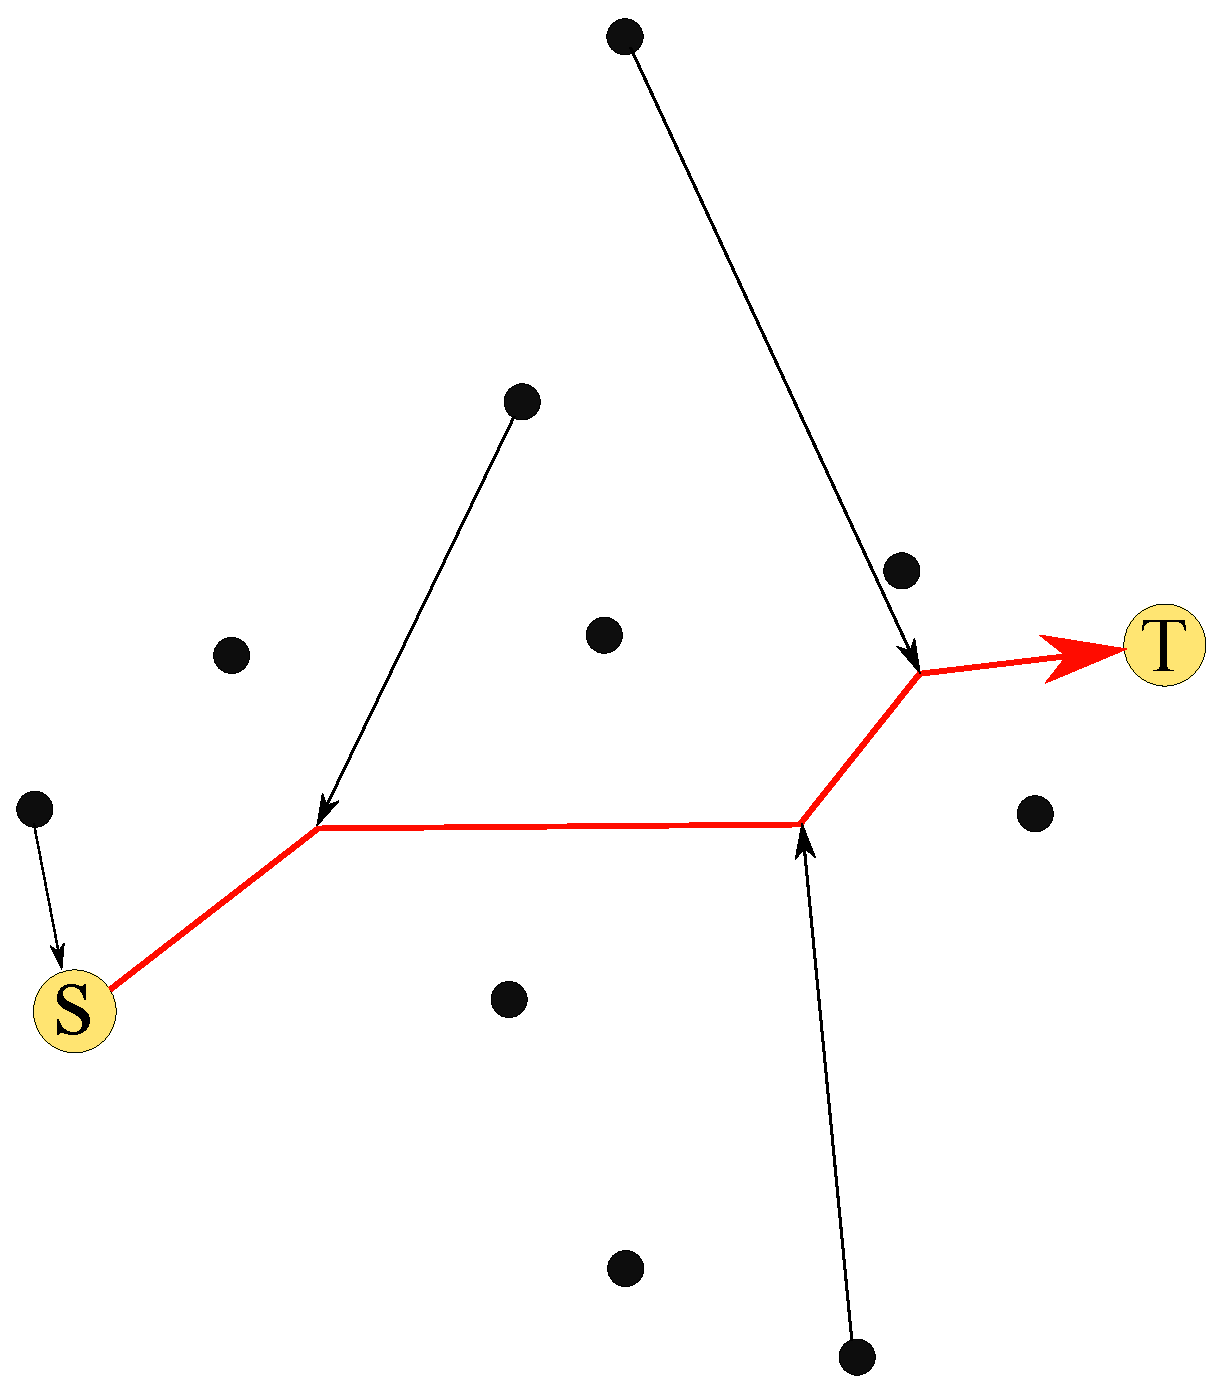
\includegraphics[width=6cm]{docs/introex.eps}
    \caption{An instance of the Package Handoff problem for a single package being transported from $S$ to $T$. 
     Agents are located at the dots marked in black. The package travels along the red path. The agents all have 
     different velocities, and in this example, assumed to have infinite battery capacity.}%
    \label{fig:introex}%
  \end{center}
\end{wrapfigure}

How do you get a package from an initial location $S$ to a destination point $T$ using a fleet of ``heterogenous'' carrier agents 
(e.g. drones, taxis). By ``heterogenous'' we mean the two agents can have different capabilities like 
different maximum speed or different fuel capacity. 


In the simplest version of the category of problems, 
we are given as input the initial locations of $n$  agents in $\mathbb{R}^2$ 
each capable of a maximum speed $u_i >0$ (where $u_i$ need not be equal to $v_j$ for $i \neq j$).
Each agent can pick up the package and move to another point to \textit{rendezvous with} and 
\textit{hand off} the 
package to another agent. This other agent then either proceeds to $T$ or decides to meet with 
and hand off the package to another agent \footnote{If it makes the package get to $T$ faster} 
and so on and so forth. 

The objective is to get the agents to cooperate to send the package from $S$ to $T$ in the 
least possible time. We call this the \textit{Package Handoff Problem}. 

To solve this problem and its various avatars 
\footnote{Say when there are multiple packages to be delivered or a bound on fuel} 
we need to 


\begin{enumerate}
\item Figure out which subset $S = \{i_1, i_2, \ldots i_k\}$ of the drones are used in the optimal schedule. 
\item Find the order in which the handoffs happend between the drones used in a schedule. 
\item Calculate the ``handoff'' points where drone $i_m$ hands over the package to drone $i_{m+1}$ 
\footnote{The last drone in the computed schedule, of course, flies directly to $T$}
\end{enumerate}

A real world instance of the basic Package Handoff problem, as described in the abstract, is when a 
ride hailing service  must co-ordinate its fleet of taxis to transport a passenger from a given location 
in the quickest possible time to the target destination on the map. In this model, 
a passenger ``hops rides'' when two taxis meet: a taxi first gets to the passenger and takes him/her to 
a point where it rendezvous with another taxi, at which point the passenger swaps taxis. This process continues 
until the passenger hops onto a taxi that goes straight to the target.  

This package handoff process is depicted in \autoref{fig:introex}. 


\section{A note on source code}
Many of the heuristics algorithms described here are implemented as literate programs \cite{Knuth:1984:LP:473.479} 
in Python 2.7.12 using the NuWeb tool \cite{briggs1992nuweb} available from \url{http://nuweb.sourceforge.net/}
alongside associated theoretical and empirical analysis. All the algorithmic code goes into the 
file \verb|pholib.py|, and any associated helper codes go into the files which are named as \verb|utils_*.py|. 
The code for these utility files has been given in the appendices. 

The \verb|pholib.py| file looks like 

%{python-mode}%
\begin{flushleft} \small\label{scrap1}\raggedright\small
\NWtarget{nuweb3}{} \verb@"src/pholib.py"@\nobreak\ {\footnotesize {3}}$\equiv$
\vspace{-1ex}
\begin{list}{}{} \item
\mbox{}\verb@@\\
\mbox{}\verb@from colorama import Fore, Style@\\
\mbox{}\verb@from matplotlib import rc@\\
\mbox{}\verb@import matplotlib as mpl@\\
\mbox{}\verb@import matplotlib.pyplot as plt@\\
\mbox{}\verb@from scipy.optimize import minimize@\\
\mbox{}\verb@from sklearn.cluster import KMeans@\\
\mbox{}\verb@import numpy as np@\\
\mbox{}\verb@import argparse, inspect, itertools, logging@\\
\mbox{}\verb@import os, time, sys@\\
\mbox{}\verb@import pprint as pp, randomcolor @\\
\mbox{}\verb@import utils_algo, utils_graphics@\\
\mbox{}\verb@@\\
\mbox{}\verb@@\hbox{$\langle\,${\itshape Algorithms}\nobreak\ {\footnotesize \NWlink{nuweb7}{7}}$\,\rangle$}\verb@@\\
\mbox{}\verb@@\hbox{$\langle\,${\itshape Experiments}\nobreak\ {\footnotesize ?}$\,\rangle$}\verb@@\\
\mbox{}\verb@@\hbox{$\langle\,${\itshape Run Handlers}\nobreak\ {\footnotesize \NWlink{nuweb20}{20}}$\,\rangle$}\verb@@\\
\mbox{}\verb@@\hbox{$\langle\,${\itshape Plotting}\nobreak\ {\footnotesize \NWlink{nuweb24}{24}}$\,\rangle$}\verb@@\\
\mbox{}\verb@@{\NWsep}
\end{list}
\vspace{-1.5ex}
\footnotesize
\begin{list}{}{\setlength{\itemsep}{-\parsep}\setlength{\itemindent}{-\leftmargin}}

\item{}
\end{list}
\vspace{4ex}
\end{flushleft}
%{/python-mode}%

The chapters are devoted to fleshing out the chunks \textlangle \verb|Algorithms|\textrangle and 
\textlangle\verb|Experiments|\textrangle.  The \newline \textlangle \verb|Run Handlers|\textrangle and 
\textlangle \verb|Plotting|\textrangle \; chunks is mainly to deal with interactive matplotlib input, 
and as such are boring and banished to the Appendix \Winkey . 

All source code files are tangled to the \verb|src| directory. The point of entry for the code are 
\verb|main*.py| which are implemented separately in the \verb|src| directory, since their contents 
can change based on what library code is being called 
for during development and testing. Since these files are very short and the mechanics clear, 
they are implemented as standalone files (i.e. not inside this document) but directly in the \verb|src| folder 
itself. To run the code in interactive mode run the code as \verb|python src/main_interactive.py| on a 
Unix / Windows terminal in the root folder of the project \footnote{This code has been tested on an 64 bit 
machine running Linux Mint 18.3 (Sylvia) running the Linux Kernel version 4.10.0-38-generic with an 
Intel(R) Core(TM) i7 CPU 960 @ 3.20GHz CPU}. 

For a short overview of previous work on this problem see Appendix 

Each of the following sections correspond to a fixed variant of the package handoff problem and describe
algorithms for that specific variant. Enough talk! Onto algorithms! 

\section{Unlimited Fuel, Different Drone Speeds}

Much of the machinery developed in solving this basic basic basic question will be generalized and extended to 
other variants of the package handoff problem. 

We repeat the problem definition and fix some notation that will be used for the remainder 
of the section 

\begin{displayquote}
  We are given as input the initial locations $P_i$ of $n$  agents in $\mathbb{R}^2$ 
each capable of a maximum speed $u_i >0$ (where $u_i$ need not be equal to $v_j$ for $i \neq j$).
Each agent can pick up the package and move to another point to \textit{rendezvous with} and 
\textit{hand off} the 
package to another agent. This other agent then either proceeds to $T$ or decides to meet with 
and hand off the package to another agent and so on. 
The objective is to get the agents to cooperate to send the package from $S$ to $T$ in the 
least possible time. 
\end{displayquote}

We represent the handoff points as follows $H_{i_1} \ldots H_{i_k}$ for $0 \leq i_0, \ldots i_k \leq n$ stand 
for points where the drones with labels $i_0, \ldots i_k$ hand the package off in that order. More precisely 
$H_{i_j}$ is the point where drone $i_{j-1}$ hands off the package to drone $i_j$ for $1 \leq j \leq k$.  

A solution to the package handoff problem is completely specified by computing the handoff points \textit{and} the 
drone ids involved in the exchange at each handoff point. 

The optimal schedule is denoted $OPT$. It is easy to see the statements of the following structural lemma always 
hold for $OPT$. 

\begin{flem}

In $OPT$
\begin{alphalist}
\item A package is always transferred to a faster drone at a handoff point. 
\item A drone handles a package at most once i.e. if a drone hands off the package, 
      it will never be involved in a handling that package again. 
\item All drones involved in the handoff start moving simultaneously at time $t=0$ 
\item No two drones wait at a rendezvous point before rendezvous happens. 
     \footnote{waiting can happen in other problem variants 
     say when there is limited fuel or only a finite set of 
     allowed rendezvous points}
\item The path of the package is a radially monotone piecewise straight polygonal curve with respect to the 
    direction ST no matter what the initial positions $P_i$ or speeds $u_i$ of the drones. 
\item $\frac{|ST|}{v_{max}}$ is a (trivial) lower bound for $OPT$, where $v_{max}$ denotes the speed of the fastest drone. 
\end{alphalist}
\end{flem}

\begin{proof}
\todo[inline]{TODO!}
\end{proof}

\newpage
\subsection{Handoff in a fixed order}
\label{ssec:fixorder}
If we know the drones involved in the handoff \textit{along with} the order of handoff 
then we can compute the handoff points --- and hence the path of the package --- exactly via 
convex optimization as outlined in Lemma \autoref{lem:fixorder}. This fact will be exploited in many 
heuristics: such methods will compute a subset of drones involved in the handoff (alongwith 
the handoff order) followed by a call to the convex program. 


\begin{figure}[H]
\centering
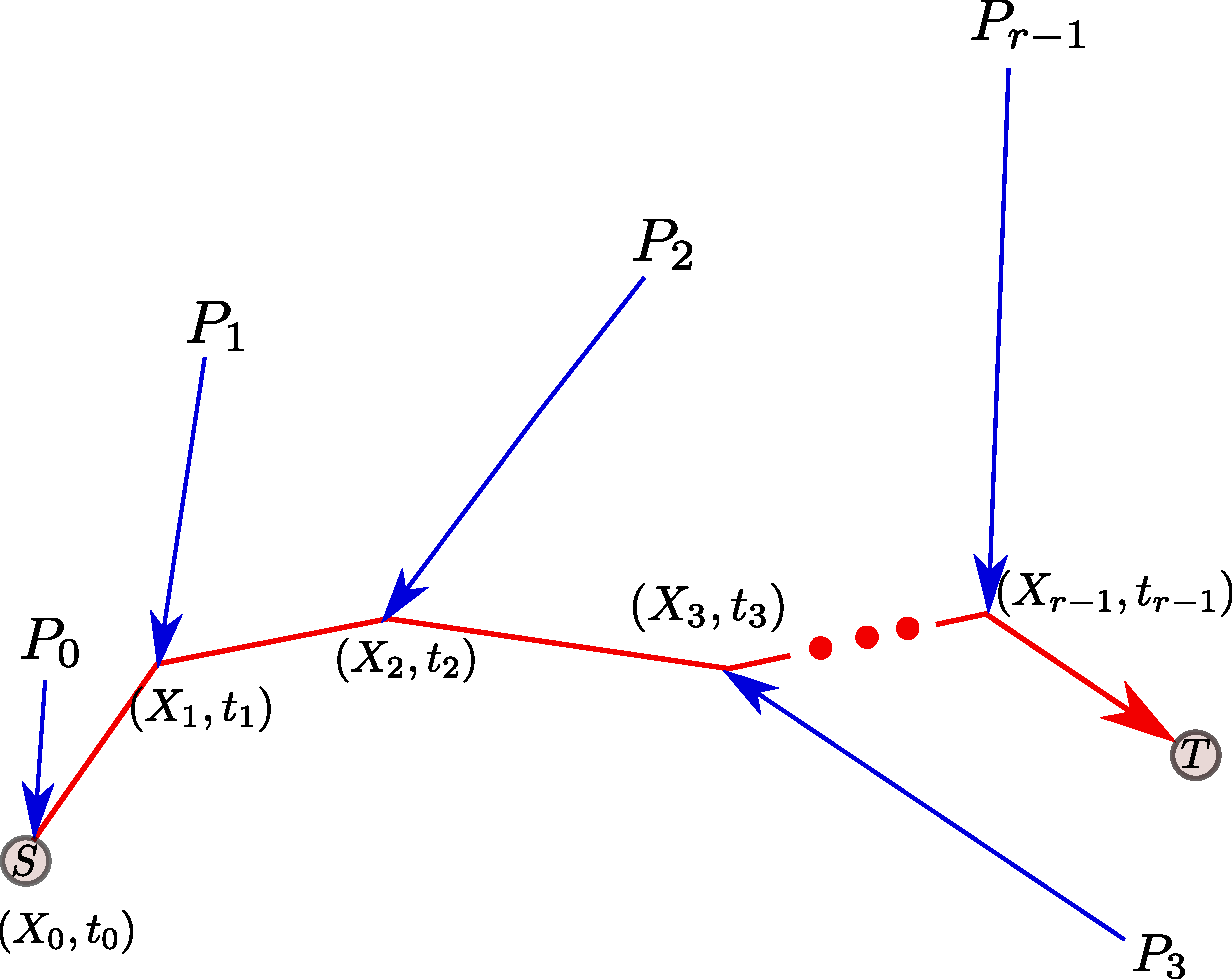
\includegraphics[width=8cm]{docs/pho-cvx.pdf}
\caption{The path of the package is shown in red. The drones invovled in the handoff are 
labelled $P_i$ in the prespecified handoff order.}
\end{figure}
\label{fig:fixorder}

\begin{flem} \label{lem:fixorder}
Given as input are drones with initial positions $P_i \in \RR^2$, with speeds $u_i>0$ 
for  $1 \leq i \leq r-1$, the intial position $S$ and final destination $T$ 
for the package. \footnote{See \autoref{fig:fixorder} for an illustration of the notation used in this lemma} 
The drones are expected to transport the package by handing of the package in the order $1,2,\ldots, r$.
Let $t_i$ denote the departure time on a global clock from the $i$'th handoff point $X_i$. 

Then the minimum time and handoff points for transporting the package and the handoff points 
can be calculated by the following convex program

\begin{equation*}
\min_{t_i, X_i} \; \; \; t_{r-1} + \frac{||T-X_{r-1}||}{u_{r-1}}
\end{equation*}

subject to the constraints

\begin{align*}
X_0 &= S\\  
t_i &\geq \frac{||P_i-X_i||}{u_i} \qquad \qquad 0 \leq i \leq r-1\\
t_i + \frac{||X_{i+1}-X_i||}{u_i} &\leq t_{i+1} \qquad \qquad \qquad \;\;\;\; 0 \leq i \leq r-2
\end{align*}

\end{flem}

\begin{proof}
\todo[inline]{TODO!}
\end{proof}

The following function is just an implentation of the convex program just described. 
Here \verb|drone_info| is a list 
of tuples, where each tuple consits of the initial position and speed of the drone. The order of the 
drones is assumed to be that in which the list of drones is provided. \verb|source| and \verb|target|
are just coordinate locations of $S$ and $T$ respectively. We use the CVXPY \cite{cvxpy} library 
as a black-box convex optimization solver. 

%{python-mode}%
\begin{flushleft} \small\label{scrap2}\raggedright\small
\NWtarget{nuweb7}{} $\langle\,${\itshape Algorithms}\nobreak\ {\footnotesize {7}}$\,\rangle\equiv$
\vspace{-1ex}
\begin{list}{}{} \item
\mbox{}\verb@def algo_pho_exact_given_order_of_drones ( drone_info, source, target ):@\\
\mbox{}\verb@    import cvxpy as cp@\\
\mbox{}\verb@@\\
\mbox{}\verb@    source = np.asarray(source)@\\
\mbox{}\verb@    target = np.asarray(target)@\\
\mbox{}\verb@@\\
\mbox{}\verb@    r = len(drone_info) @\\
\mbox{}\verb@    source = np.asarray(source)@\\
\mbox{}\verb@    target = np.asarray(target)@\\
\mbox{}\verb@    @\\
\mbox{}\verb@    # Variables for rendezvous points of drone with package@\\
\mbox{}\verb@    X, t = [], []@\\
\mbox{}\verb@    for i in range(r):@\\
\mbox{}\verb@       X.append(cp.Variable(2)) # vector variable@\\
\mbox{}\verb@       t.append(cp.Variable( )) # scalar variable@\\
\mbox{}\verb@@\\
\mbox{}\verb@    # Constraints @\\
\mbox{}\verb@    constraints_S = [  X[0] == source ]@\\
\mbox{}\verb@@\\
\mbox{}\verb@    constraints_I = [] @\\
\mbox{}\verb@    for i in range(r):@\\
\mbox{}\verb@      constraints_I.append(0.0 <= t[i])@\\
\mbox{}\verb@      constraints_I.append(t[i] >= cp.norm(np.asarray(drone_info[i][0])-X[i])/drone_info[i][1])@\\
\mbox{}\verb@@\\
\mbox{}\verb@    constraints_L = []@\\
\mbox{}\verb@    for i in range(r-1):@\\
\mbox{}\verb@      constraints_L.append(t[i] + cp.norm(X[i+1] - X[i])/drone_info[i][1] <= t[i+1])@\\
\mbox{}\verb@@\\
\mbox{}\verb@    objective = cp.Minimize(t[r-1]+cp.norm(target-X[r-1])/drone_info[r-1][1])@\\
\mbox{}\verb@@\\
\mbox{}\verb@    prob = cp.Problem(objective, constraints_S + constraints_I + constraints_L)@\\
\mbox{}\verb@    print Fore.CYAN@\\
\mbox{}\verb@    prob.solve(solver=cp.SCS,verbose=True)@\\
\mbox{}\verb@    print Style.RESET_ALL@\\
\mbox{}\verb@    @\\
\mbox{}\verb@    package_trail = [ np.asarray(X[i].value) for i in range(r) ] + [ target ]@\\
\mbox{}\verb@    return package_trail@\\
\mbox{}\verb@@{\NWsep}
\end{list}
\vspace{-1.5ex}
\footnotesize
\begin{list}{}{\setlength{\itemsep}{-\parsep}\setlength{\itemindent}{-\leftmargin}}
\item \NWtxtMacroRefIn\ \NWlink{nuweb3}{3}.

\item{}
\end{list}
\vspace{4ex}
\end{flushleft}
%{/python-mode}%


We next describe a heuristic that use Continuous Dijkstra \cite{mitchell2000geometric} 
type approach in computing approximate solutions to $OPT$.

\subsection{One Dimensional Greedy Wavefront}
\label{ssec:odw}

In this heuristic we first constrain the package to travel along the line $\vec{ST}$, then compute the 
subset of the drones involved in the schedule, and finally pass of the list of drones involved to the convex
program given in Lemma \autoref{lem:fixorder} to calculate the rendezvous points. 


\begin{figure}[H]
\centering
   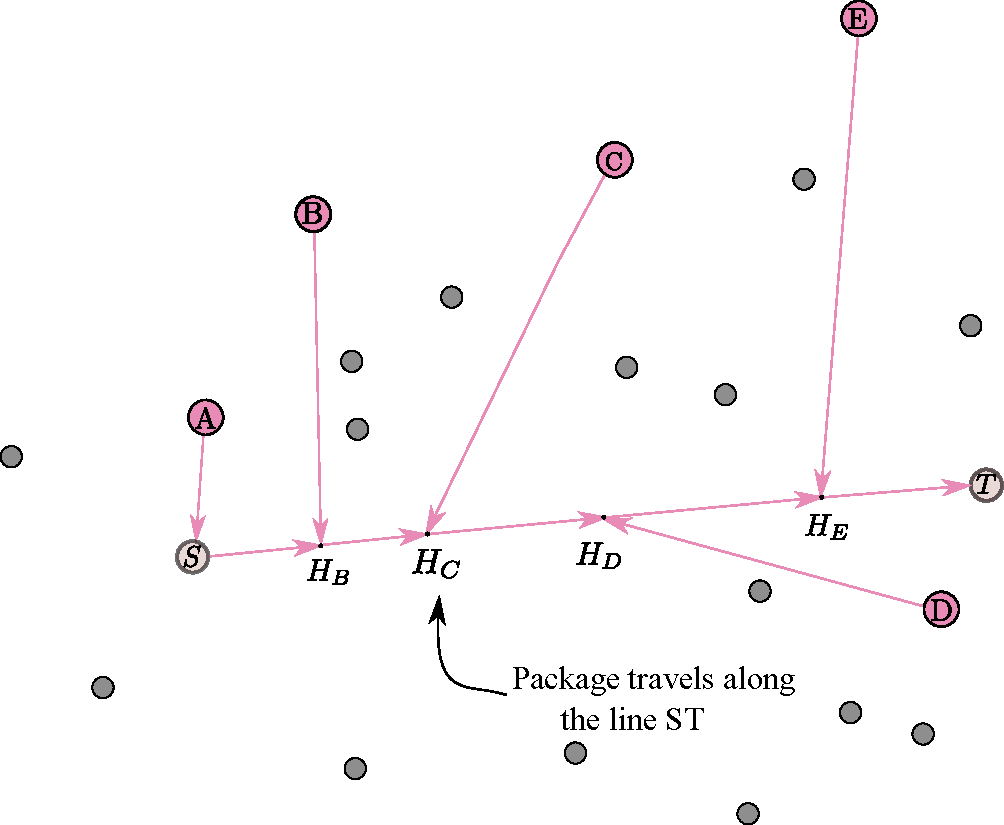
\includegraphics[width=14cm]{docs/straight-line-pho-ex.pdf}
    \caption{The package travels along the straight line $\vec{ST}$. The point where drone $A$ hands off the 
     package to drone $B$ depicted as $H_B$, and similarly for other drones. Drones involved in the handoff 
     are marked in pink. Those not involved are marked in gray. Two drones may have different speed.}
\end{figure}



\begin{algorithm}[H]
\DontPrintSemicolon % Some LaTeX compilers require you to use \dontprintsemicolon instead 
\KwIn{
\begin{enumerate}
\item Coordinates of initial position of source $S$ and target $T$ of the package.
\item Coordinates of the onitial positions $P_i$ of each drone $1 \leq i \leq n$.
\item Maximum possible speed $u_i$ of each drone $1 \leq i \leq n$. 
\end{enumerate}

}
\KwOut{

\begin{enumerate}
 \item  \myblue{$t^*$}: The time required for the package to get from $S$ to $T$.
 \item  \myblue{$L = (i_1, i_2, \ldots, i_k)$} : An ordered list of indices of the drones involved in the handoff. 
 \item \myblue{$\mathcal{H} =  \{ \, S \, \} \cup \{ \, H_{i_j} \mid j\geq 2  \, \}$}:  An ordered list of handoff points.
$H_{i_j} \in \RR^2$ is where the drone with index $i_j$ picks up the package 
       \textit{from} drone $i_{j-1}$. 
\end{enumerate}
}

\vspace{4mm}

$t \gets 0$ \tcp*[h]{Time on the global clock} \;
$wavelets \gets [ (i, 0) \mid 0 \leq i \leq n ]$ \tcp*[h]{Active Wavelets: indices and current radius}\;

\vspace{2mm}
\tcc*[h]{Find first wavelet to reach $S$ and update $wavelets$} \;

\tcc*[h]{Start wavelet expansion from $S$} \;
\For{$i \gets 1$ \textbf{to} $r$}{
  \While{$n \geq c_i$} {
    $C \gets C \cup \{c_i\}$   \;
    $n \gets n - c_i$ 
  }
}
\Return{$t^*, L, \mathcal{H}$}\;
\caption{{\sc One dimensional greedy wavefront}}
\label{algo:odgw}
\end{algorithm}

\begin{figure}[H]
\centering
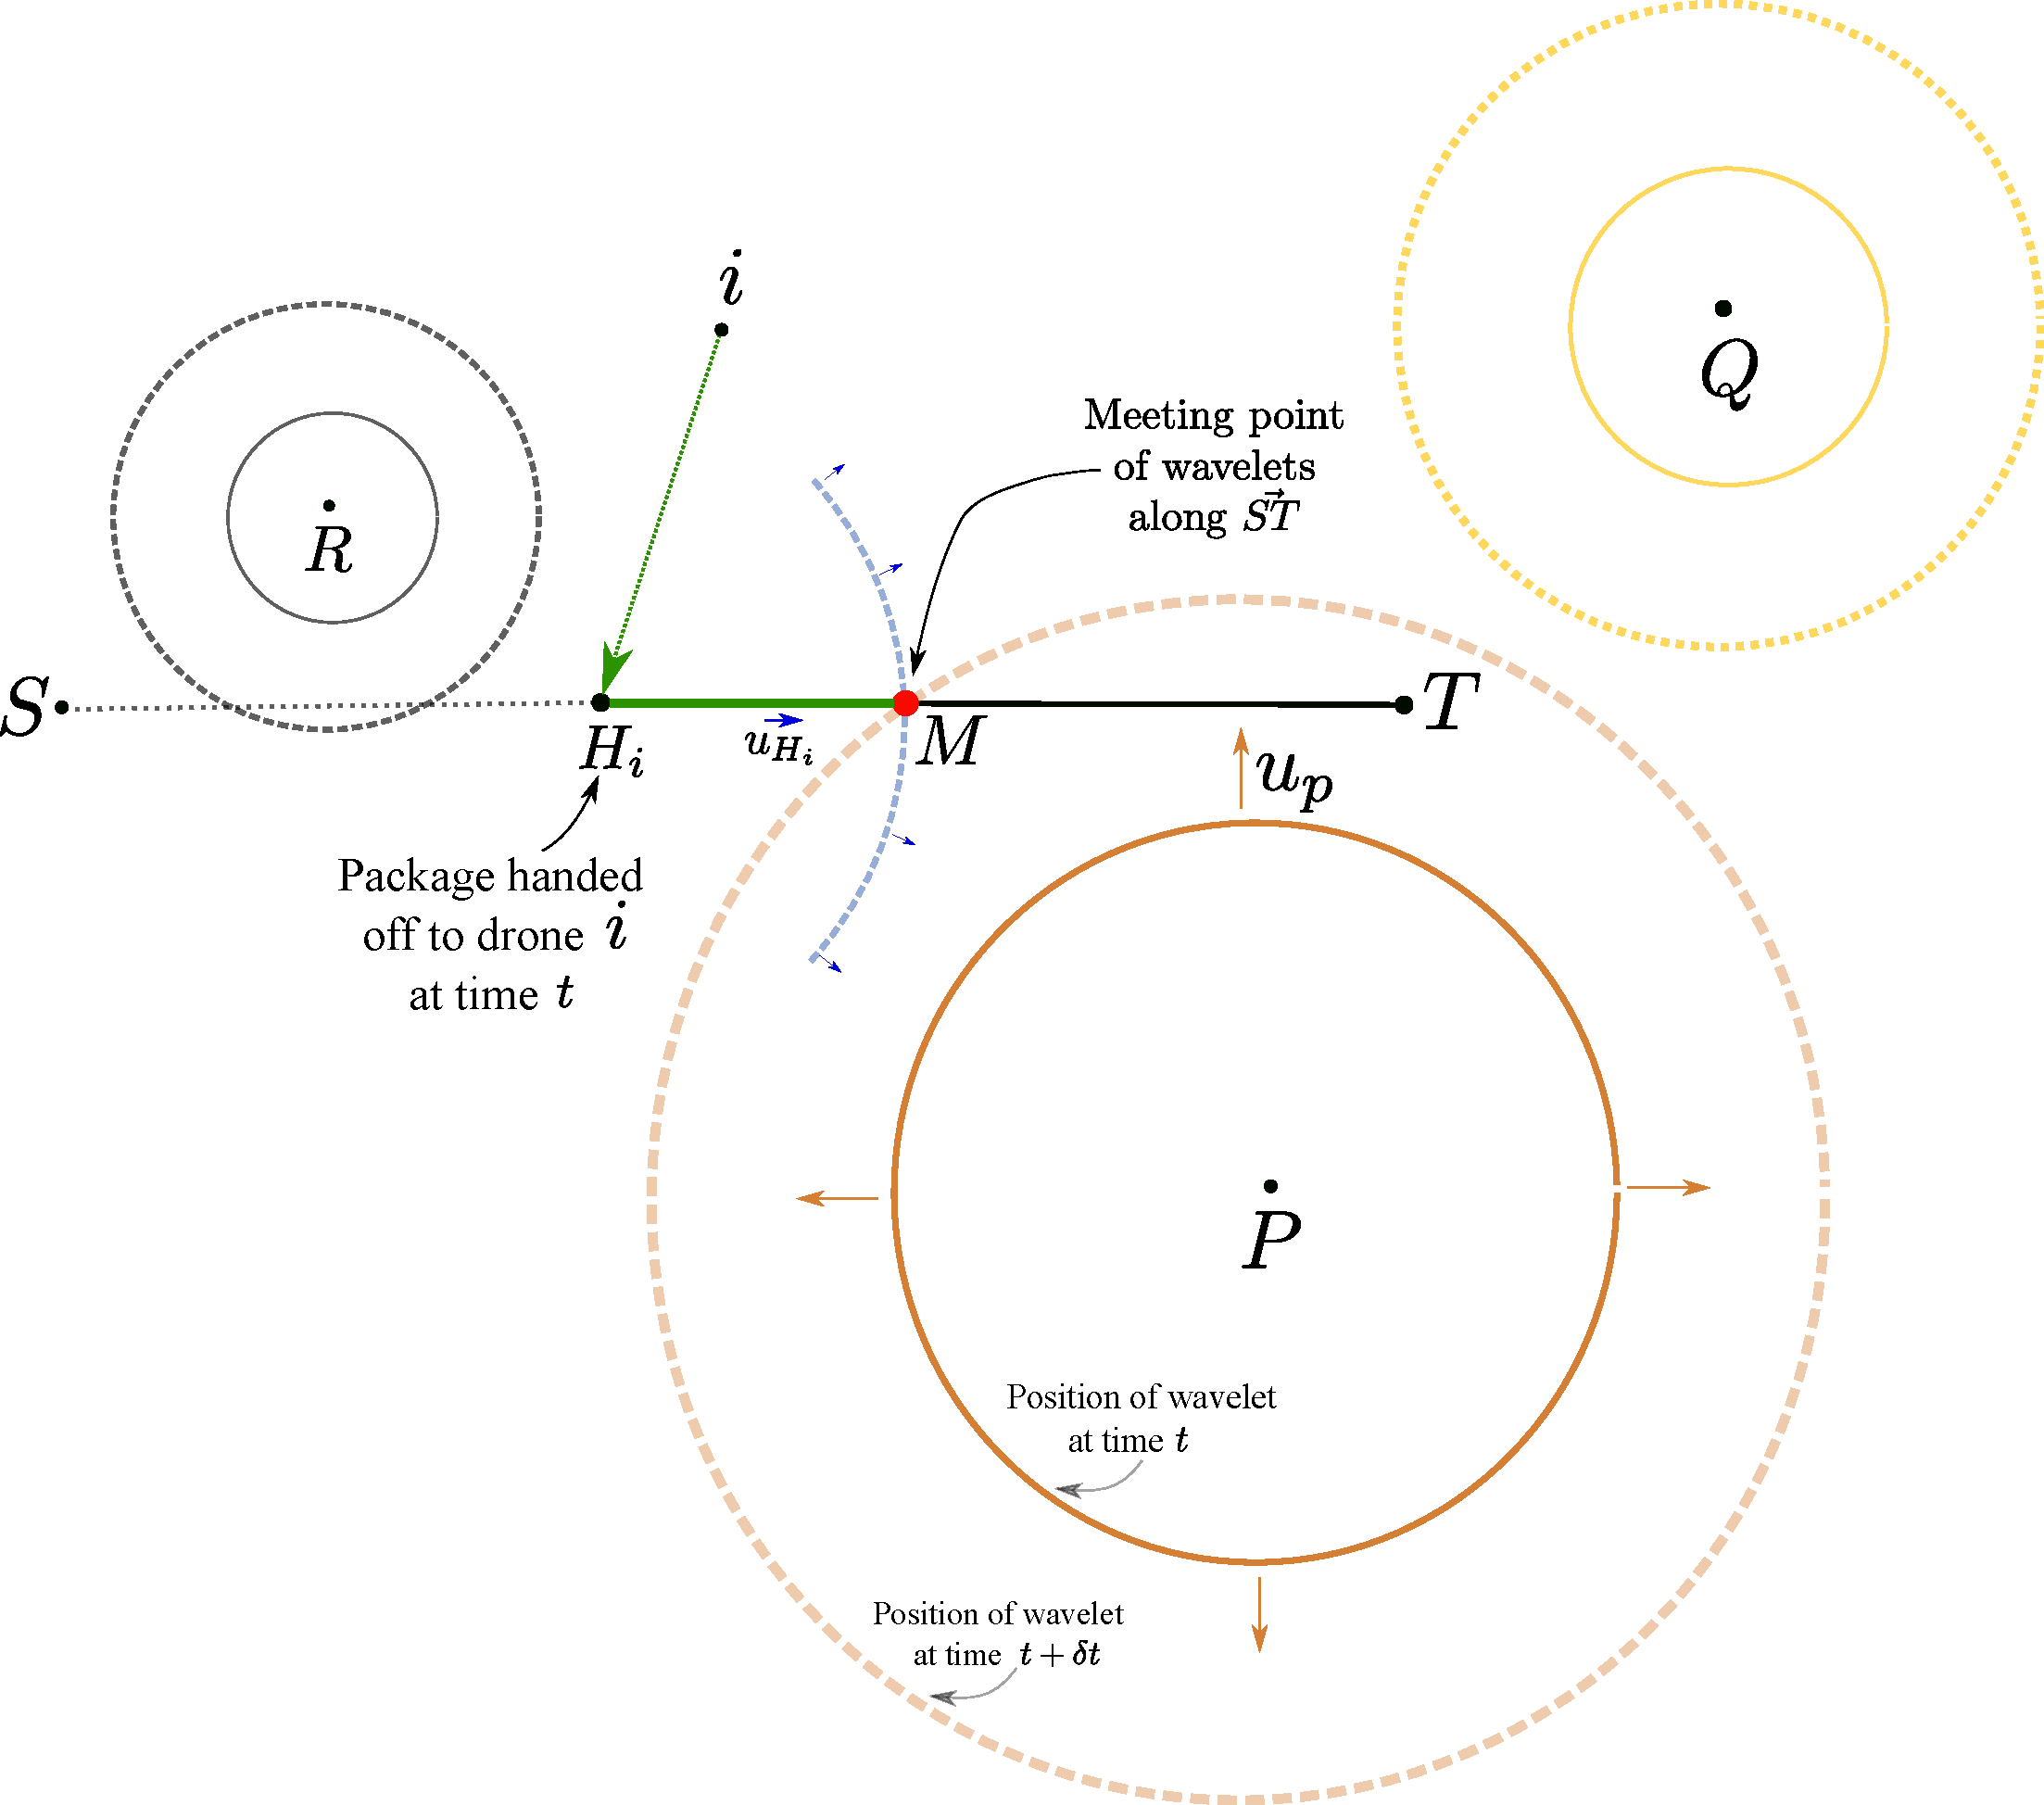
\includegraphics[width=12cm]{docs/circular_wavelets_intersect_along_st.pdf}
\caption{Intersection of two expanding wavelets along $\vec{H_iT}$. The figure shows  snapshots of two times;
one at time $t$ when the package has just been handed off to drone $i$ at $H_i$ and another at time $t + \delta t$
when a wavelet corresponding a drone faster than drone $i$ meets the wavelet expanding from $H_i$ with speed $u_i$ 
at $M$}
\end{figure}

\newpage
\nocite{*}
\printbibliography
\begin{appendices}

\chapter{History and Previous Work}


\begin{wrapfigure}{L}{0.5\textwidth}
  \begin{center}
      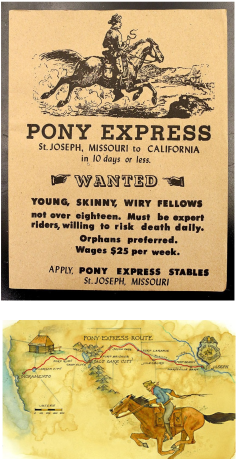
\includegraphics[width=6cm]{docs/pony-express.png}
      \caption{A job application poster and a relay route used for the Pony Express. 
      Images taken from \cite{orphans} and \cite{ponyroute} respectively.}
  \end{center}
\end{wrapfigure}

A system of using relays for delivering packages is not a particularly new idea. A 
famous (and shortlived!) example of such a relay system was the Pony Express company which 
was used a system of a relay of horse riders tp transport mail from St. Joseph, Missouri to 
Sacramento, California. 

To quote the Wikipedia article

\begin{quote}

\textit{``Operated by Central Overland California and Pike's Peak Express Company, the Pony Express was a great 
financial investment to the U.S. During its 18 months of operation, it reduced the time for messages to travel 
between the Atlantic and Pacific coasts to about 10 days. It became the West's most direct means of east-west 
communication before the transcontinental telegraph was established (October 24, 1861), and was vital for tying 
the new U.S. state of California with the rest of the United States.The Pony Express demonstrated that a unified 
transcontinental system of communications could be established and operated year-round. ''}
\end{quote}


While the invention of the telegraph might have run the Pony Express out of business, the idea of using relay agents 
such as drones --- instead of horses! --- to transfer packages can have applications today for sending physical goods 
(which of course can't be telegraphed! \Winkey) such as  life-saving medicinces in under-developed 
countries or in disaster relief areas. 
ZipLine\cite{zipline} \cite{zipline-ted} and Matternet \cite{matternet} are just two of the companies which 
are involved in building networks of drones for precisely such missions.

\begin{figure}[H]
  \centering
  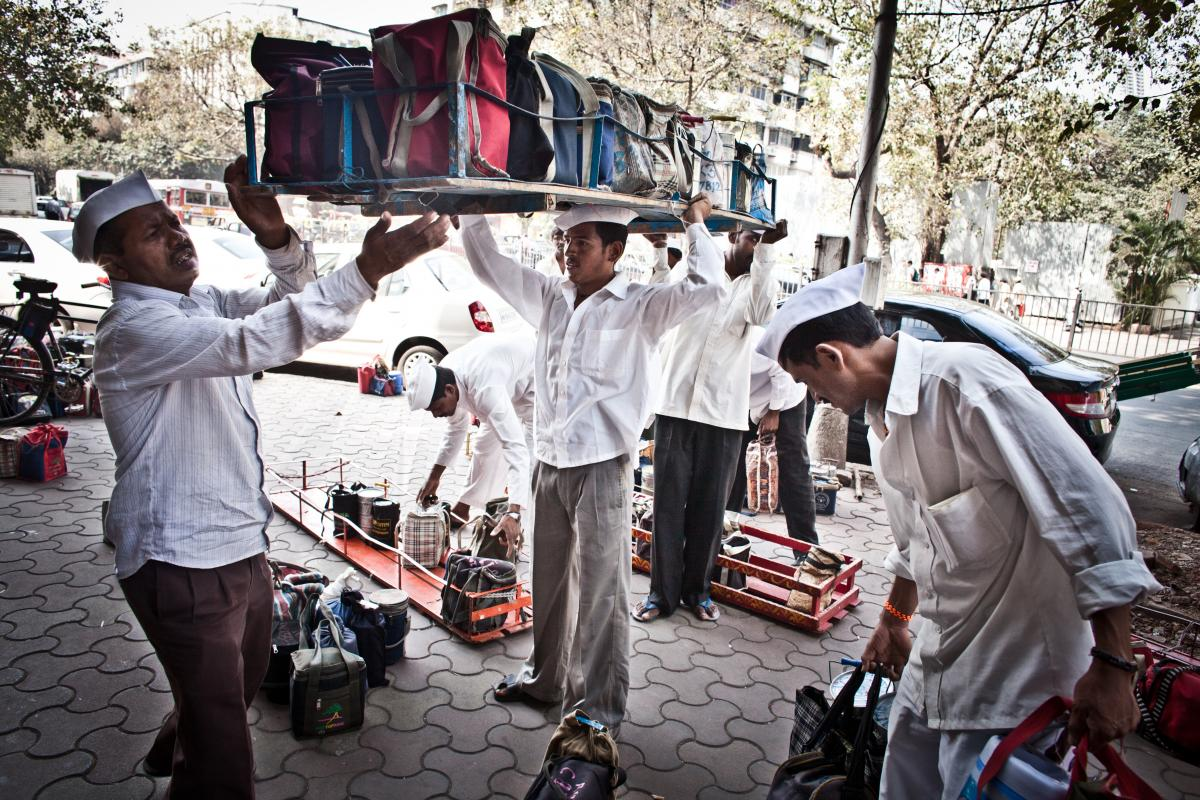
\includegraphics[width=12cm]{docs/dabba.jpg}
  \caption{Dabbawallas exchanging lunchboxes (dabbas) at a relay point. Image from \cite{Magazine2019Oct} }
\end{figure}


Another relay system for package deliveries (135 years old and still functioning!) is that of 
the \textit{dabbawallas} \footnote{literally: lunchbox carriers} used for transporting lunch boxes from 
homes and restaurants to people at work in Mumbai, India. To quote from \cite{dabba}
\begin{quote}
\textit{Four thousand five hundred semi-literate dabbawalas collect and deliver 175,000 packages 
within hours. What should we learn from this unique, simple and highly efficient 120-year-old 
logistics system? [\ldots] After the customer leaves for work, her lunch is packed into a tiffin 
provided by the dabbawala. A color-coded notation on the handle identifies its owner and destination. 
Once the dabbawala has picked up the tiffin, he moves fast using a combination of bicycles, trains and his 
two feet.}

\textit{A BBC crew filming dabbawalas in action was amazed at their speed. ``Following our dabbawala 
wasn't easy, our film crew quickly lost him in the congestion of the train station. At Victoria 
Terminus we found other fast moving dabbawalas, but not our subject... and at Mr Bhapat's ayurvedic 
pharmacy, the lunch had arrived long before the film crew,'' the documentary noted wryly. So, how do 
they work so efficiently?}

\textit{The entire system depends on teamwork and meticulous timing. Tiffins are collected from homes 
between 7.00 am and 9.00 am, and taken to the nearest railway station. At various intermediary stations, 
they are hauled onto platforms and sorted out for area-wise distribution, so that a single tiffin could 
change hands three to four times in the course of its daily journey.}

\textit{At Mumbai's downtown stations, the last link in the chain, a final relay of dabbawalas fan 
out to the tiffins' destined bellies. Lunch hour over, the whole process moves into reverse and the 
tiffins return to suburban homes by 6.00 pm.}
\end{quote}

See \url{https://youtu.be/dX-0el2wuEU} for a short video on the dabbawallas. 

\chapter{\texttt{utils\char`_graphics.py}}

This file contains useful functions for visualization and plotting functions described in the previous chapters.
%{python-mode}%
\begin{flushleft} \small\label{scrap3}\raggedright\small
\NWtarget{nuweb15}{} \verb@"src/utils_graphics.py"@\nobreak\ {\footnotesize {15}}$\equiv$
\vspace{-1ex}
\begin{list}{}{} \item
\mbox{}\verb@    @\\
\mbox{}\verb@from matplotlib import rc@\\
\mbox{}\verb@from colorama import Fore@\\
\mbox{}\verb@from colorama import Style@\\
\mbox{}\verb@from scipy.optimize import minimize@\\
\mbox{}\verb@from sklearn.cluster import KMeans@\\
\mbox{}\verb@import argparse@\\
\mbox{}\verb@import itertools@\\
\mbox{}\verb@import math@\\
\mbox{}\verb@import matplotlib as mpl@\\
\mbox{}\verb@import matplotlib.pyplot as plt@\\
\mbox{}\verb@import numpy as np@\\
\mbox{}\verb@import os@\\
\mbox{}\verb@import pprint as pp@\\
\mbox{}\verb@import randomcolor @\\
\mbox{}\verb@import sys@\\
\mbox{}\verb@import time@\\
\mbox{}\verb@@\\
\mbox{}\verb@xlim, ylim = [0,1], [0,1]@\\
\mbox{}\verb@@\\
\mbox{}\verb@# Borrowed from https://stackoverflow.com/a/9701141@\\
\mbox{}\verb@import numpy as np@\\
\mbox{}\verb@import colorsys@\\
\mbox{}\verb@@\\
\mbox{}\verb@def get_colors(num_colors, lightness=0.2):@\\
\mbox{}\verb@    colors=[]@\\
\mbox{}\verb@    for i in np.arange(60., 360., 300. / num_colors):@\\
\mbox{}\verb@        hue        = i/360.0@\\
\mbox{}\verb@        saturation = 0.95@\\
\mbox{}\verb@        colors.append(colorsys.hls_to_rgb(hue, lightness, saturation))@\\
\mbox{}\verb@    return colors@\\
\mbox{}\verb@@{\NWsep}
\end{list}
\vspace{-1.5ex}
\footnotesize
\begin{list}{}{\setlength{\itemsep}{-\parsep}\setlength{\itemindent}{-\leftmargin}}

\item{}
\end{list}
\vspace{4ex}
\end{flushleft}
%{/python-mode}%

\newpage

\chapter{\texttt{utils\char`_algo.py}}

This file contains useful functions for writing algorithms described in the previous chapters.

%{python-mode}%
\begin{flushleft} \small\label{scrap4}\raggedright\small
\NWtarget{nuweb17}{} \verb@"src/utils_algo.py"@\nobreak\ {\footnotesize {17}}$\equiv$
\vspace{-1ex}
\begin{list}{}{} \item
\mbox{}\verb@@\\
\mbox{}\verb@ import numpy as np@\\
\mbox{}\verb@import random@\\
\mbox{}\verb@from colorama import Fore@\\
\mbox{}\verb@from colorama import Style@\\
\mbox{}\verb@@\\
\mbox{}\verb@def vector_chain_from_point_list(pts):@\\
\mbox{}\verb@    vec_chain = []@\\
\mbox{}\verb@    for pair in zip(pts, pts[1:]):@\\
\mbox{}\verb@        tail= np.array (pair[0])@\\
\mbox{}\verb@        head= np.array (pair[1])@\\
\mbox{}\verb@        vec_chain.append(head-tail)@\\
\mbox{}\verb@@\\
\mbox{}\verb@    return vec_chain@\\
\mbox{}\verb@@\\
\mbox{}\verb@def length_polygonal_chain(pts):@\\
\mbox{}\verb@    vec_chain = vector_chain_from_point_list(pts)@\\
\mbox{}\verb@@\\
\mbox{}\verb@    acc = 0@\\
\mbox{}\verb@    for vec in vec_chain:@\\
\mbox{}\verb@        acc = acc + np.linalg.norm(vec)@\\
\mbox{}\verb@    return acc@\\
\mbox{}\verb@def pointify_vector (x):@\\
\mbox{}\verb@    if len(x) % 2 == 0:@\\
\mbox{}\verb@        pts = []@\\
\mbox{}\verb@        for i in range(len(x))[::2]:@\\
\mbox{}\verb@            pts.append( [x[i],x[i+1]] )@\\
\mbox{}\verb@        return pts@\\
\mbox{}\verb@    else :@\\
\mbox{}\verb@        sys.exit('List of items does not have an even length to be able to be pointifyed')@\\
\mbox{}\verb@def flatten_list_of_lists(l):@\\
\mbox{}\verb@       return [item for sublist in l for item in sublist]@\\
\mbox{}\verb@def print_list(xs):@\\
\mbox{}\verb@    for x in xs:@\\
\mbox{}\verb@        print x@\\
\mbox{}\verb@def partial_sums( xs ):@\\
\mbox{}\verb@    psum = 0@\\
\mbox{}\verb@    acc = []@\\
\mbox{}\verb@    for x in xs:@\\
\mbox{}\verb@        psum = psum+x@\\
\mbox{}\verb@        acc.append( psum )@\\
\mbox{}\verb@    return acc@\\
\mbox{}\verb@def are_site_orderings_equal(sites1, sites2):@\\
\mbox{}\verb@@\\
\mbox{}\verb@    for (x1,y1), (x2,y2) in zip(sites1, sites2): @\\
\mbox{}\verb@        if (x1-x2)**2 + (y1-y2)**2 > 1e-8:@\\
\mbox{}\verb@            return False@\\
\mbox{}\verb@    return True@\\
\mbox{}\verb@def bunch_of_non_uniform_random_points(numpts):@\\
\mbox{}\verb@    cluster_size = int(np.sqrt(numpts)) @\\
\mbox{}\verb@    numcenters   = cluster_size@\\
\mbox{}\verb@    @\\
\mbox{}\verb@    import scipy@\\
\mbox{}\verb@    import random@\\
\mbox{}\verb@    centers = scipy.rand(numcenters,2).tolist()@\\
\mbox{}\verb@@\\
\mbox{}\verb@    scale, points = 4.0, []@\\
\mbox{}\verb@    for c in centers:@\\
\mbox{}\verb@        cx, cy = c[0], c[1]@\\
\mbox{}\verb@        # For current center $c$ of this loop, generate \verb|cluster_size| points uniformly in a square centered at it@\\
\mbox{}\verb@           @\\
\mbox{}\verb@        sq_size      = min(cx,1-cx,cy, 1-cy)@\\
\mbox{}\verb@        loc_pts_x    = np.random.uniform(low=cx-sq_size/scale, high=cx+sq_size/scale, size=(cluster_size,))@\\
\mbox{}\verb@        loc_pts_y    = np.random.uniform(low=cy-sq_size/scale, high=cy+sq_size/scale, size=(cluster_size,))@\\
\mbox{}\verb@        points.extend(zip(loc_pts_x, loc_pts_y))@\\
\mbox{}\verb@        @\\
\mbox{}\verb@@\\
\mbox{}\verb@    # Whatever number of points are left to be generated, generate them uniformly inside the unit-square@\\
\mbox{}\verb@       @\\
\mbox{}\verb@    num_remaining_pts = numpts - cluster_size * numcenters@\\
\mbox{}\verb@    remaining_pts = scipy.rand(num_remaining_pts, 2).tolist()@\\
\mbox{}\verb@    points.extend(remaining_pts)@\\
\mbox{}\verb@    @\\
\mbox{}\verb@@\\
\mbox{}\verb@    return points@\\
\mbox{}\verb@    @\\
\mbox{}\verb@def write_to_yaml_file(data, dir_name, file_name):@\\
\mbox{}\verb@   import yaml@\\
\mbox{}\verb@   with open(dir_name + '/' + file_name, 'w') as outfile:@\\
\mbox{}\verb@     yaml.dump( data, outfile, default_flow_style = False)@\\
\mbox{}\verb@@{\NWsep}
\end{list}
\vspace{-1.5ex}
\footnotesize
\begin{list}{}{\setlength{\itemsep}{-\parsep}\setlength{\itemindent}{-\leftmargin}}

\item{}
\end{list}
\vspace{4ex}
\end{flushleft}
%{/python-mode}%

\chapter{Implementation of \textlangle \texttt{Run Handlers}\textrangle}

This chunk contains code required for the interactive input of sites and agents onto the canvas. 

%{python-mode}%
\begin{flushleft} \small\label{scrap5}\raggedright\small
\NWtarget{nuweb20}{} $\langle\,${\itshape Run Handlers}\nobreak\ {\footnotesize {20}}$\,\rangle\equiv$
\vspace{-1ex}
\begin{list}{}{} \item
\mbox{}\verb@@\\
\mbox{}\verb@@\\
\mbox{}\verb@class Single_PHO_Input:@\\
\mbox{}\verb@    def __init__(self, drone_info = [] , source = None, target=None):@\\
\mbox{}\verb@           self.drone_info = drone_info @\\
\mbox{}\verb@           self.source     = source@\\
\mbox{}\verb@           self.target     = target@\\
\mbox{}\verb@@\\
\mbox{}\verb@    def get_drone_pis (self):@\\
\mbox{}\verb@           return [self.drone_info[idx][0] for idx in range(len(self.drone_info)) ]@\\
\mbox{}\verb@           @\\
\mbox{}\verb@    def get_drone_uis (self):@\\
\mbox{}\verb@           return [self.drone_info[idx][1] for idx in range(len(self.drone_info)) ]@\\
\mbox{}\verb@         @\\
\mbox{}\verb@    def get_tour(self, algo, animate_tour_p=False, plot_tour_p=False):@\\
\mbox{}\verb@           return algo( self.drone_info, @\\
\mbox{}\verb@                        self.source, @\\
\mbox{}\verb@                        self.target, @\\
\mbox{}\verb@                        animate_tour_p, @\\
\mbox{}\verb@                        plot_tour_p    )@\\
\mbox{}\verb@@\\
\mbox{}\verb@    # Methods for \verb|ReverseHorseflyInput|@\\
\mbox{}\verb@    def clearAllStates (self):@\\
\mbox{}\verb@          self.drone_info = []@\\
\mbox{}\verb@          self.source = None@\\
\mbox{}\verb@          self.target = None@\\
\mbox{}\verb@@\\
\mbox{}\verb@def single_pho_run_handler():@\\
\mbox{}\verb@    import random@\\
\mbox{}\verb@    def wrapperEnterRunPoints(fig, ax, run):@\\
\mbox{}\verb@      def _enterPoints(event):@\\
\mbox{}\verb@        if event.name      == 'button_press_event'          and \@\\
\mbox{}\verb@           (event.button   == 1 or event.button == 3)       and \@\\
\mbox{}\verb@            event.dblclick == True and event.xdata  != None and event.ydata  != None:@\\
\mbox{}\verb@@\\
\mbox{}\verb@             if event.button == 1:  @\\
\mbox{}\verb@                 # Insert blue circle representing the initial position of a drone@\\
\mbox{}\verb@                 print Fore.GREEN@\\
\mbox{}\verb@                 newPoint = (event.xdata, event.ydata)@\\
\mbox{}\verb@                 speed    = np.random.uniform() # float(raw_input('What speed do you want for the drone at '+str(newPoint)))@\\
\mbox{}\verb@                 run.drone_info.append( (newPoint, speed) ) @\\
\mbox{}\verb@                 patchSize  = (xlim[1]-xlim[0])/40.0@\\
\mbox{}\verb@                 print Style.RESET_ALL@\\
\mbox{}\verb@                 @\\
\mbox{}\verb@                 ax.add_patch( mpl.patches.Circle( newPoint, radius = patchSize,@\\
\mbox{}\verb@                                                   facecolor='#b7e8cc', edgecolor='black'  ))@\\
\mbox{}\verb@@\\
\mbox{}\verb@                 ax.text( newPoint[0], newPoint[1], "{:.2f}".format(speed), fontsize=15, @\\
\mbox{}\verb@                          horizontalalignment='center', verticalalignment='center' )@\\
\mbox{}\verb@@\\
\mbox{}\verb@                 ax.set_title('Number of drones inserted: ' +\@\\
\mbox{}\verb@                              str(len(run.drone_info)), fontdict={'fontsize':25})@\\
\mbox{}\verb@                 @\\
\mbox{}\verb@             elif event.button == 3:  @\\
\mbox{}\verb@                 # Insert big red circles representing the source and target points@\\
\mbox{}\verb@                 patchSize  = (xlim[1]-xlim[0])/50.0@\\
\mbox{}\verb@                 if run.source is None:    @\\
\mbox{}\verb@                      run.source = (event.xdata, event.ydata)  @\\
\mbox{}\verb@                      ax.add_patch( mpl.patches.Circle( run.source, radius = patchSize, @\\
\mbox{}\verb@                                                        facecolor= '#ffd9d6', edgecolor='black', lw=1.0 ))@\\
\mbox{}\verb@                      ax.text( run.source[0], run.source[1], 'S', fontsize=15, @\\
\mbox{}\verb@                               horizontalalignment='center', verticalalignment='center' )@\\
\mbox{}\verb@@\\
\mbox{}\verb@                 elif run.target is None:@\\
\mbox{}\verb@                      run.target = (event.xdata, event.ydata)  @\\
\mbox{}\verb@                      ax.add_patch( mpl.patches.Circle( run.target, radius = patchSize, @\\
\mbox{}\verb@                                                       facecolor= '#ffd9d6', edgecolor='black', lw=1.0 ))@\\
\mbox{}\verb@                      ax.text( run.target[0], run.target[1], 'T', fontsize=15, @\\
\mbox{}\verb@                               horizontalalignment='center', verticalalignment='center' )@\\
\mbox{}\verb@                 else:@\\
\mbox{}\verb@                       print Fore.RED, "Source and Target already set", Style.RESET_ALL@\\
\mbox{}\verb@             # Clear polygon patches and set up last minute \verb|ax| tweaks@\\
\mbox{}\verb@             clearAxPolygonPatches(ax)@\\
\mbox{}\verb@             applyAxCorrection(ax)@\\
\mbox{}\verb@             fig.canvas.draw()@\\
\mbox{}\verb@      return _enterPoints@\\
\mbox{}\verb@@\\
\mbox{}\verb@    # The key-stack argument is mutable! I am using this hack to my advantage.@\\
\mbox{}\verb@    def wrapperkeyPressHandler(fig, ax, run): @\\
\mbox{}\verb@           def _keyPressHandler(event):@\\
\mbox{}\verb@               if event.key in ['i', 'I']:  @\\
\mbox{}\verb@@\\
\mbox{}\verb@                    # Select algorithm to execute@\\
\mbox{}\verb@                    algo_str = raw_input(Fore.YELLOW                                             +\@\\
\mbox{}\verb@                            "Enter algorithm to be used to compute the tour:\n Options are:\n"   +\@\\
\mbox{}\verb@                            " (odw)     One Dimensional Wavefront \n"                            +\@\\
\mbox{}\verb@                            Style.RESET_ALL)@\\
\mbox{}\verb@@\\
\mbox{}\verb@                    algo_str = algo_str.lstrip()@\\
\mbox{}\verb@                     @\\
\mbox{}\verb@                    # Incase there are patches present from the previous clustering, just clear them@\\
\mbox{}\verb@                    clearAxPolygonPatches(ax)@\\
\mbox{}\verb@                    if   algo_str == 'odw':@\\
\mbox{}\verb@                          tour = run.get_tour( algo_odw, plot_tour_p=True )@\\
\mbox{}\verb@                    else:@\\
\mbox{}\verb@                          print "Unknown option. No horsefly for you! ;-D "@\\
\mbox{}\verb@                          sys.exit()@\\
\mbox{}\verb@                    applyAxCorrection(ax)@\\
\mbox{}\verb@                    fig.canvas.draw()@\\
\mbox{}\verb@                    @\\
\mbox{}\verb@               elif event.key in ['c', 'C']: @\\
\mbox{}\verb@                    # Clear canvas and states of all objects@\\
\mbox{}\verb@                    run.clearAllStates()@\\
\mbox{}\verb@                    ax.cla()@\\
\mbox{}\verb@                                  @\\
\mbox{}\verb@                    applyAxCorrection(ax)@\\
\mbox{}\verb@                    ax.set_xticks([])@\\
\mbox{}\verb@                    ax.set_yticks([])@\\
\mbox{}\verb@                                     @\\
\mbox{}\verb@                    fig.texts = []@\\
\mbox{}\verb@                    fig.canvas.draw()@\\
\mbox{}\verb@           return _keyPressHandler@\\
\mbox{}\verb@    @\\
\mbox{}\verb@    # Set up interactive canvas@\\
\mbox{}\verb@    fig, ax =  plt.subplots()@\\
\mbox{}\verb@    run = Single_PHO_Input()@\\
\mbox{}\verb@        @\\
\mbox{}\verb@    from matplotlib import rc@\\
\mbox{}\verb@    @\\
\mbox{}\verb@    # specify the custom font to use@\\
\mbox{}\verb@    plt.rcParams['font.family'] = 'sans-serif'@\\
\mbox{}\verb@    plt.rcParams['font.sans-serif'] = 'Times New Roman'@\\
\mbox{}\verb@@\\
\mbox{}\verb@    ax.set_xlim([xlim[0], xlim[1]])@\\
\mbox{}\verb@    ax.set_ylim([ylim[0], ylim[1]])@\\
\mbox{}\verb@    ax.set_aspect(1.0)@\\
\mbox{}\verb@    ax.set_xticks([])@\\
\mbox{}\verb@    ax.set_yticks([])@\\
\mbox{}\verb@          @\\
\mbox{}\verb@    ax.set_title("Enter drone positions, source and target onto canvas. \n \@\\
\mbox{}\verb@(Enter speeds into the terminal, after inserting a drone at a particular position)")@\\
\mbox{}\verb@@\\
\mbox{}\verb@    mouseClick   = wrapperEnterRunPoints (fig,ax, run)@\\
\mbox{}\verb@    fig.canvas.mpl_connect('button_press_event' , mouseClick)@\\
\mbox{}\verb@          @\\
\mbox{}\verb@    keyPress     = wrapperkeyPressHandler(fig,ax, run)@\\
\mbox{}\verb@    fig.canvas.mpl_connect('key_press_event', keyPress   )@\\
\mbox{}\verb@    @\\
\mbox{}\verb@    plt.show()@\\
\mbox{}\verb@@{\NWsep}
\end{list}
\vspace{-1.5ex}
\footnotesize
\begin{list}{}{\setlength{\itemsep}{-\parsep}\setlength{\itemindent}{-\leftmargin}}
\item \NWtxtMacroRefIn\ \NWlink{nuweb3}{3}.

\item{}
\end{list}
\vspace{4ex}
\end{flushleft}
%{/python-mode}%

\chapter{Implementation of \textlangle\texttt{Plotting}\textrangle}

We typically plot the tours onto a separate window if the boolean switch \verb|plot_tour_p| 
is set to \verb|True| while calling the algorithm. The path of the package is shown in bold red. 
The paths of the drones from their initial positions to the point where they pick up the package 
from another drone are shown in blue.

An example output from the \verb|plot_tour| function is shown below.

\begin{figure}[H]
\centering
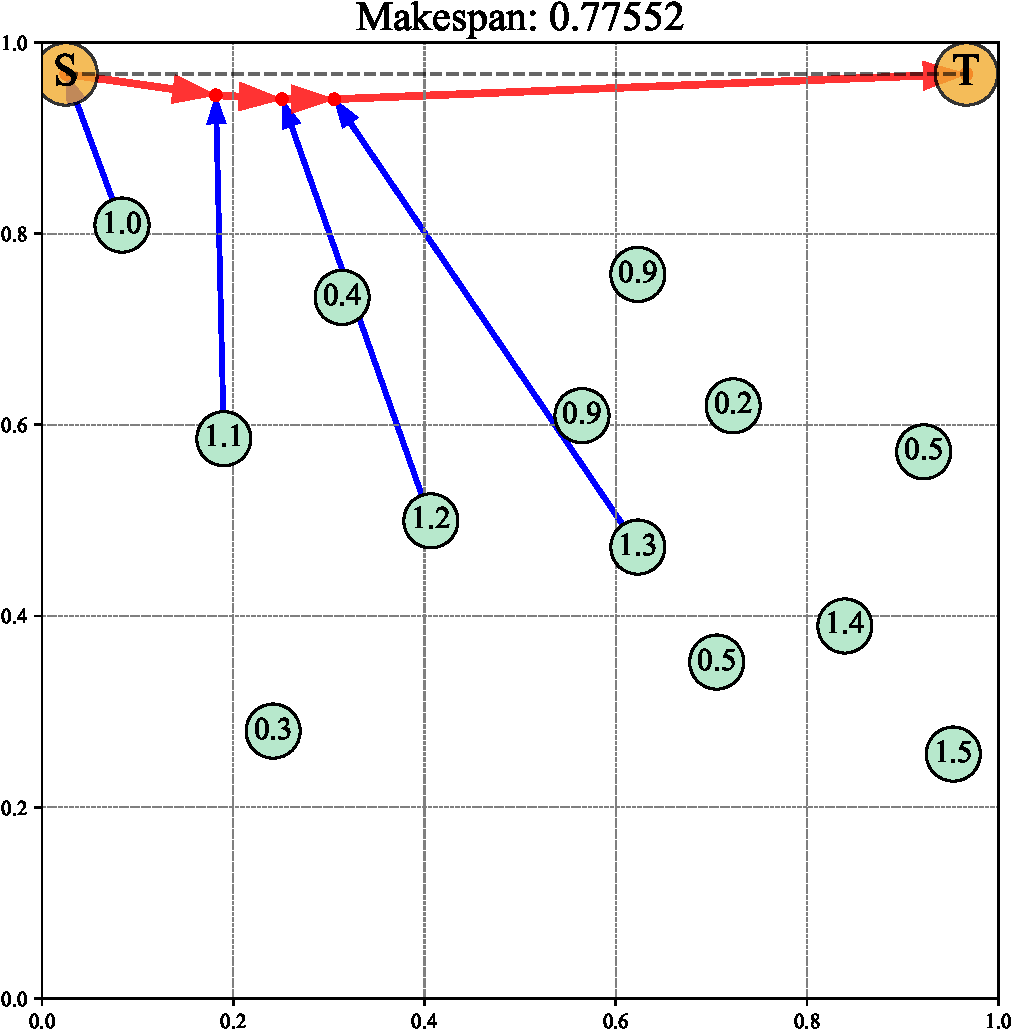
\includegraphics[width=8cm]{docs/pho_example_plot.pdf}
\caption{The numbers inside the circle indicate the speed of the drone}
\end{figure}

%{python-mode}%
\begin{flushleft} \small\label{scrap6}\raggedright\small
\NWtarget{nuweb24}{} $\langle\,${\itshape Plotting}\nobreak\ {\footnotesize {24}}$\,\rangle\equiv$
\vspace{-1ex}
\begin{list}{}{} \item
\mbox{}\verb@@\\
\mbox{}\verb@def plot_tour(fig, ax, figtitle, source, target, @\\
\mbox{}\verb@              drone_info, used_drones, package_trail,@\\
\mbox{}\verb@              xlims=[0,1],@\\
\mbox{}\verb@              ylims=[0,1],@\\
\mbox{}\verb@              aspect_ratio=1.0,@\\
\mbox{}\verb@              speedfontsize=4,@\\
\mbox{}\verb@              speedmarkersize=10,@\\
\mbox{}\verb@              sourcetargetmarkerfontsize=4,@\\
\mbox{}\verb@              sourcetargetmarkersize=10 ):@\\
\mbox{}\verb@@\\
\mbox{}\verb@    import matplotlib.ticker as ticker@\\
\mbox{}\verb@    ax.set_aspect(aspect_ratio)@\\
\mbox{}\verb@    ax.set_xlim(xlims)@\\
\mbox{}\verb@    ax.set_ylim(ylims)@\\
\mbox{}\verb@@\\
\mbox{}\verb@    plt.rc('font', family='serif')@\\
\mbox{}\verb@@\\
\mbox{}\verb@    # Draw the package trail@\\
\mbox{}\verb@    xs, ys = extract_coordinates(package_trail)@\\
\mbox{}\verb@    ax.plot(xs,ys, 'ro', markersize=5 )@\\
\mbox{}\verb@    for idx in range(len(xs)-1):@\\
\mbox{}\verb@          plt.arrow( xs[idx], ys[idx], xs[idx+1]-xs[idx], ys[idx+1]-ys[idx], @\\
\mbox{}\verb@                    **{'length_includes_head': True, @\\
\mbox{}\verb@                       'width': 0.007 , @\\
\mbox{}\verb@                       'head_width':0.01, @\\
\mbox{}\verb@                       'fc': 'r', @\\
\mbox{}\verb@                       'ec': 'none',@\\
\mbox{}\verb@                       'alpha': 0.8})@\\
\mbox{}\verb@@\\
\mbox{}\verb@@\\
\mbox{}\verb@    # Draw the source, target, and initial positions of the robots as bold dots@\\
\mbox{}\verb@    xs,ys = extract_coordinates([source, target])@\\
\mbox{}\verb@    ax.plot(xs,ys, 'o', markersize=sourcetargetmarkersize, alpha=0.8, ms=10, mec='k', mfc='#F1AB30' )@\\
\mbox{}\verb@    #ax.plot(xs,ys, 'k--', alpha=0.6 ) # light line connecting source and target@\\
\mbox{}\verb@@\\
\mbox{}\verb@    ax.text(source[0], source[1], 'S', fontsize=sourcetargetmarkerfontsize,\@\\
\mbox{}\verb@            horizontalalignment='center',verticalalignment='center')@\\
\mbox{}\verb@    ax.text(target[0], target[1], 'T', fontsize=sourcetargetmarkerfontsize,\@\\
\mbox{}\verb@            horizontalalignment='center',verticalalignment='center')@\\
\mbox{}\verb@@\\
\mbox{}\verb@    xs, ys = extract_coordinates( [ drone_info[idx][0] for idx in range(len(drone_info)) ]  )@\\
\mbox{}\verb@    ax.plot(xs,ys, 'o', markersize=speedmarkersize, alpha = 0.5, mec='None', mfc='#b7e8cc' )@\\
\mbox{}\verb@@\\
\mbox{}\verb@    # Draw speed labels@\\
\mbox{}\verb@    for idx in range(len(drone_info)):@\\
\mbox{}\verb@         ax.text( drone_info[idx][0][0], drone_info[idx][0][1], format(drone_info[idx][1],'.3f'),@\\
\mbox{}\verb@                  fontsize=speedfontsize, horizontalalignment='center', verticalalignment='center' )@\\
\mbox{}\verb@@\\
\mbox{}\verb@    # Draw drone path from initial position to interception point@\\
\mbox{}\verb@    for pt, idx in zip(package_trail, used_drones):@\\
\mbox{}\verb@         initdroneposn = drone_info[idx][0]@\\
\mbox{}\verb@         handoffpoint  = pt@\\
\mbox{}\verb@    @\\
\mbox{}\verb@         xs, ys = extract_coordinates([initdroneposn, handoffpoint])@\\
\mbox{}\verb@         plt.arrow( xs[0], ys[0], xs[1]-xs[0], ys[1]-ys[0], @\\
\mbox{}\verb@                    **{'length_includes_head': True, @\\
\mbox{}\verb@                       'width': 0.005 , @\\
\mbox{}\verb@                       'head_width':0.02, @\\
\mbox{}\verb@                       'fc': 'b', @\\
\mbox{}\verb@                       'ec': 'none'})@\\
\mbox{}\verb@@\\
\mbox{}\verb@    fig.suptitle(figtitle, fontsize=15)@\\
\mbox{}\verb@    ax.set_title('\nMakespan: ' + format(makespan(drone_info, used_drones, package_trail),'.5f'), fontsize=8)@\\
\mbox{}\verb@@\\
\mbox{}\verb@    startx, endx = ax.get_xlim()@\\
\mbox{}\verb@    starty, endy = ax.get_ylim()@\\
\mbox{}\verb@@\\
\mbox{}\verb@@\\
\mbox{}\verb@    ax.tick_params(which='both', # Options for both major and minor ticks@\\
\mbox{}\verb@                top='off', # turn off top ticks@\\
\mbox{}\verb@                left='off', # turn off left ticks@\\
\mbox{}\verb@                right='off',  # turn off right ticks@\\
\mbox{}\verb@                bottom='off') # turn off bottom ticks@\\
\mbox{}\verb@    @\\
\mbox{}\verb@    # Customize the major grid@\\
\mbox{}\verb@    ax.grid(which='major', linestyle='-', linewidth='0.1', color='red')@\\
\mbox{}\verb@    ax.grid(which='minor', linestyle=':', linewidth='0.1', color='black')@\\
\mbox{}\verb@@\\
\mbox{}\verb@    #ax.xaxis.set_ticks(np.arange(startx, endx, 0.4))@\\
\mbox{}\verb@    #ax.xaxis.set_major_formatter(ticker.FormatStrFormatter('%0.1f'))@\\
\mbox{}\verb@     @\\
\mbox{}\verb@    #ax.yaxis.set_ticks(np.arange(starty, endy, 0.4))@\\
\mbox{}\verb@    #ax.yaxis.set_major_formatter(ticker.FormatStrFormatter('%0.1f'))@\\
\mbox{}\verb@@\\
\mbox{}\verb@    #plt.yticks(fontsize=5, rotation=90)@\\
\mbox{}\verb@    #plt.xticks(fontsize=5)@\\
\mbox{}\verb@@\\
\mbox{}\verb@    # A light grid@\\
\mbox{}\verb@    #plt.grid(color='0.5', linestyle='--', linewidth=0.5)@\\
\mbox{}\verb@@{\NWsep}
\end{list}
\vspace{-1.5ex}
\footnotesize
\begin{list}{}{\setlength{\itemsep}{-\parsep}\setlength{\itemindent}{-\leftmargin}}
\item \NWtxtMacroRefIn\ \NWlink{nuweb3}{3}.

\item{}
\end{list}
\vspace{4ex}
\end{flushleft}
%{/python-mode}%





\end{appendices}
%---------------------
\listoftodos
%---------------------
\end{document}
